\documentclass[compress, aspectratio=54]{beamer}
%\documentclass[notes=show]{beamer}
%\documentclass[xcolor=dvipsnames]{beamer}
\usepackage[export]{adjustbox}
\usepackage{sidecap}
\usepackage{subfig}
\usepackage{amssymb}
\usepackage{latexsym}
\usepackage{amsfonts}
\usepackage{amsmath}
\usepackage[absolute,overlay]{textpos}
\usepackage[english]{babel}
\usepackage[latin1]{inputenc}
\usepackage{subfig}
%\usepackage{times}
\usepackage[T1]{fontenc}
\usepackage{tabularx}
\newcolumntype{Y}{>{\small\raggedright\arraybackslash}X}
\usepackage{graphicx}
\usepackage{bigstrut}
\usepackage{bbm}
\usepackage{mathrsfs}
\usepackage{epsfig}
\usepackage{array}
%\usepackage{natbib}
\usepackage{hyperref}
\usepackage{caption}
\usepackage{comment}

\mode<presentation> {
%\usetheme[left,width=1.7cm]{Berkeley}
%\usetheme{default}
\usetheme{Boadilla}
  \usecolortheme[RGB={103,102,204}]{structure}
%\usecolortheme{dove}
  \useoutertheme{infolines}
  \setbeamercovered{transparent}
 }

%\usepackage[utf8]{inputenc}

% Default fixed font does not support bold face
\DeclareFixedFont{\ttb}{T1}{txtt}{bx}{n}{12} % for bold
\DeclareFixedFont{\ttm}{T1}{txtt}{m}{n}{12}  % for normal

% Custom colors
\usepackage{color}
\definecolor{deepblue}{rgb}{0,0,0.5}
\definecolor{deepred}{rgb}{0.6,0,0}
\definecolor{deepgreen}{rgb}{0,0.5,0}

\usepackage{listings}

% Python style for highlighting
\newcommand\pythonstyle{\lstset{
language=Python,
basicstyle=\ttm,
otherkeywords={self},             % Add keywords here
keywordstyle=\ttb\color{deepblue},
emph={MyClass,__init__},          % Custom highlighting
emphstyle=\ttb\color{deepred},    % Custom highlighting style
stringstyle=\color{deepgreen},
frame=tb,                         % Any extra options here
showstringspaces=false            % 
}}


% Python environment
\lstnewenvironment{python}[1][]
{
\pythonstyle
\lstset{#1}
}
{}

% Python for external files
\newcommand\pythonexternal[2][]{{
\pythonstyle
\lstinputlisting[#1]{#2}}}

% Python for inline
\newcommand\pythoninline[1]{{\pythonstyle\lstinline!#1!}}
%\renewcommand{\familydefault}{cmss}
%\renewcommand{\mathrm}{\mathsf}
%\renewcommand{\textrm}{\textsf}
\usefonttheme{serif}
\newcommand{\X}{{\mathbf{X}}}
\newcommand{\x}{{\mathbf{x}}}
\newcommand{\E}{\mathsf{E}}
\newcommand{\V}{\mathsf{Var}}

\DeclareGraphicsExtensions{.jpg,.pdf,.mps,.png}

\setbeamercolor{bibliography entry title}{fg=black}
\setbeamercolor{bibliography entry author}{fg=black}
\setbeamercolor{subsection in toc}{fg=structure}
\setbeamercolor{palette primary}{bg=structure, fg=white}
%\setbeamercolor{palette secondary}{bg=structure, fg=black}
%\setbeamercolor{palette tertiary}{bg=structure, fg=black}
\setbeamercolor{caption name}{fg=black} \setbeamersize{text margin
left=.8cm} \setbeamersize{text margin right=1cm}
\hypersetup{linkbordercolor={1 0 0}} \setbeamertemplate{navigation
symbols}{} \setbeamertemplate{headline}[default]

\setbeamertemplate{enumerate items}[default]

\newcounter{transfct}
\newcounter{begbs}
\newcounter{endbs}


\title[Introduction]{Introduction to Python}

\author[Arieda Mu\c co]{Arieda Mu\c co}
\institute[CEU]{Central European University}

\AtBeginSection[] {
  \begin{frame}<handout:0>
    \frametitle{TOC}
    \tableofcontents[currentsection]
  \end{frame}
}

\date{}

\pgfdeclareimage[height=.7cm]{logo}{rgs2}
\logo{\pgfuseimage{logo}}
\begin{document}
\captionsetup[subfigure]{labelformat=empty}

\frame{\titlepage}

%%%%%%%%%%%%%%%%%%%%%%%%%%%%%%%%%%%%%%%%%%%


\begin{frame}
\frametitle{Information}
\begin{itemize}
\item My research focuses on two areas: Political and Development Economics. In my research, I deal with tons of data and (lots of) text data -> programming with Python. That's why this course.
\item Introduce yourself. What are your expectations? Why are you here? What kind of data you are currently using or plan to use? 
\end{itemize}
\end{frame}
%----------------------------------------------------------------------------%

\begin{frame}
\frametitle{Plan for this course}
\begin{itemize}
\item Introduction to Python foundations
\item Introduction to  foundations of Natural Language Processing -- concepts tightly linked to Machine Learning and Artificial Intelligence

\end{itemize}
\end{frame}
%----------------------------------------------------------------------------%






%----------------------------------------------------------------------------%





%----------------------------------------------------------------------------%
\begin{frame}
\frametitle{Academic Papers in Economics}

\begin{center}
    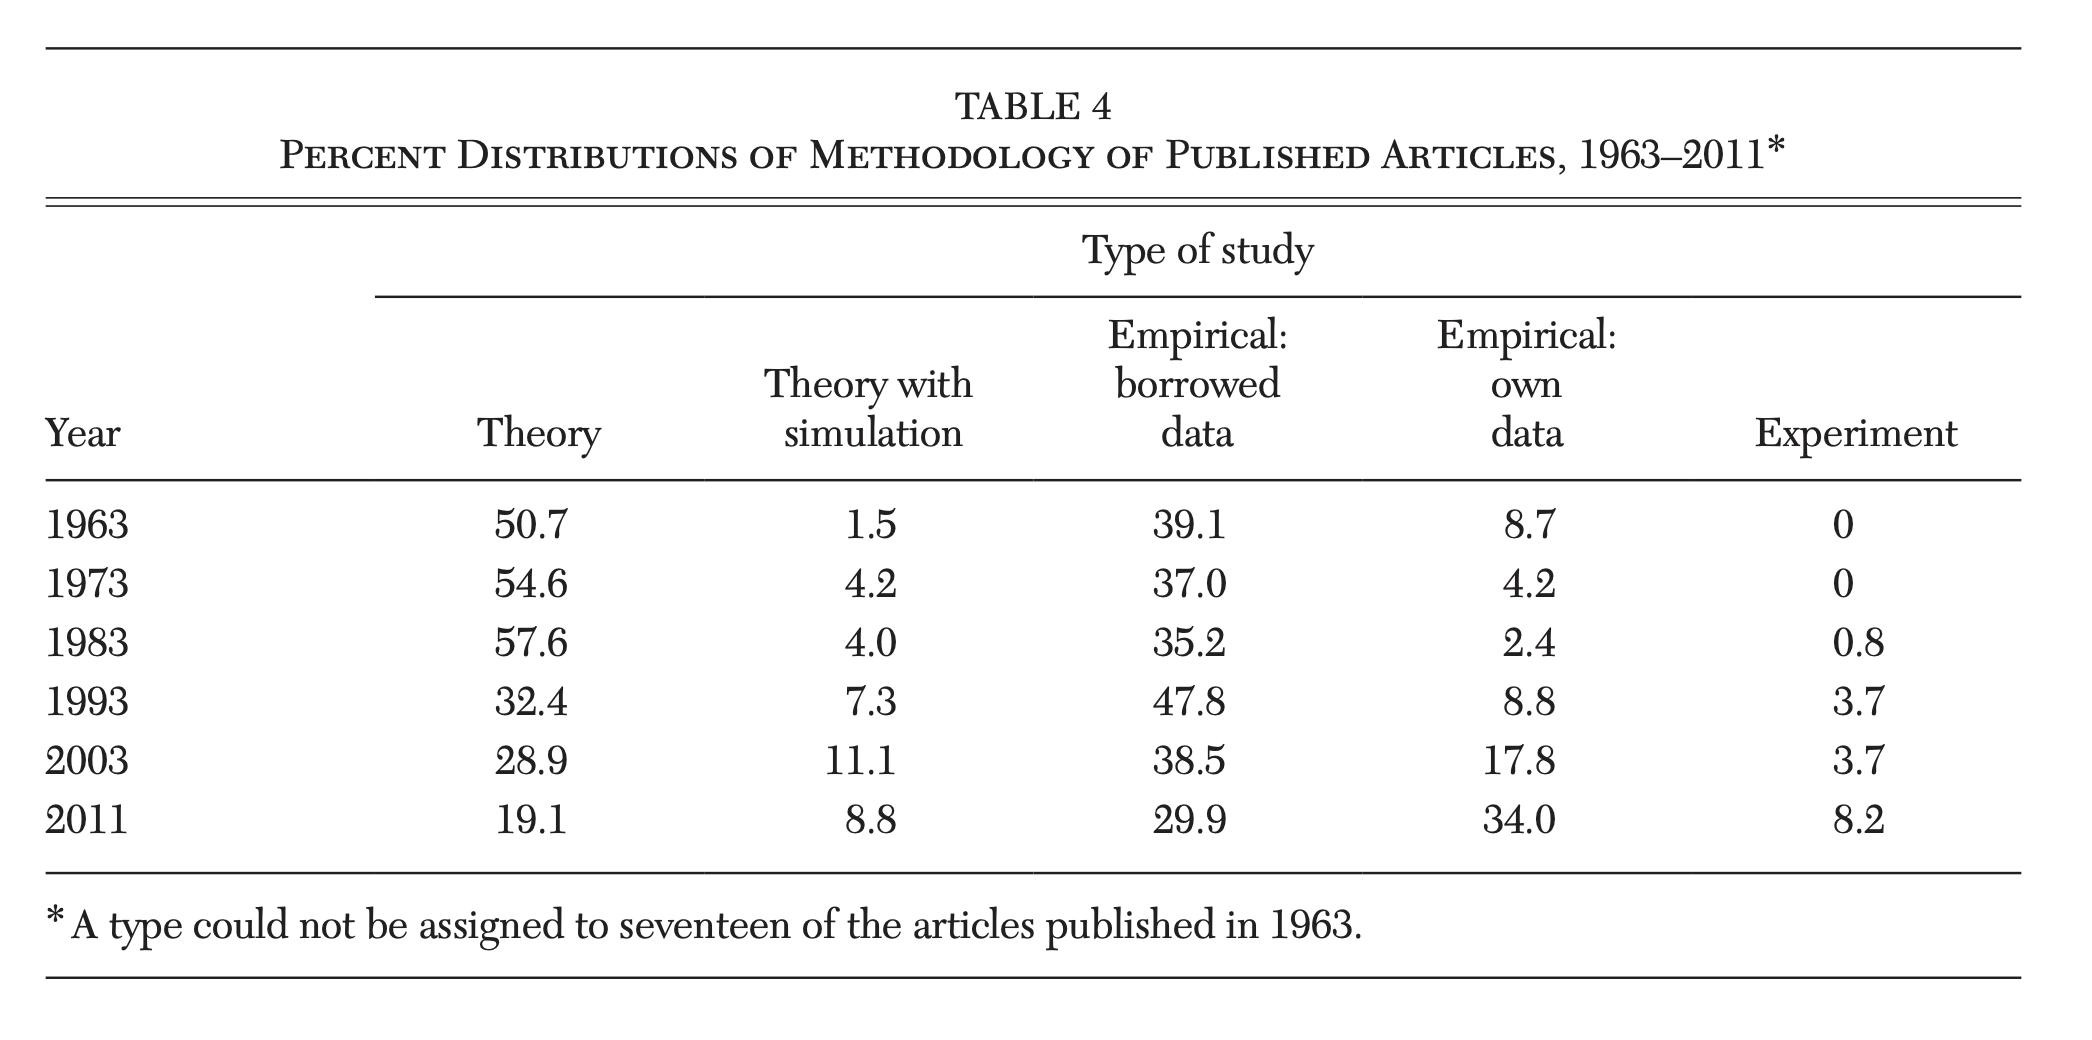
\includegraphics[width=0.8\textwidth]{Figures/percent-distribution.png}
\end{center}
Hammermesh (2013)
\end{frame}
%----------------------------------------------------------------------------%
\begin{frame}
\frametitle{Background}
\begin{itemize}
\item Old data, structured and small: (gdp, population, investment)
\item New data, less structure and larger (scraped data, consumer search patterns, social networks, texts, images, audio, video...)
\item New methods needed: data collection/management, workflow/collaboration, description/analysis

\end{itemize}
\end{frame}

%----------------------------------------------------------------------------%
\begin{frame}
\frametitle{Causal Inference and Machine Learning}
\begin{itemize}
\item Causal Inference
\begin{itemize}

\item Focus on one/few coefficients of interest (causal effect)
\item Use one main specification, show robustness to alternative specification and placebo tests
\item Model rarely evaluated (when pure inference we focus on in-sample-properties, mostly $R^2$)
\end{itemize}

\item Machine Learning (ML)
\begin{itemize}

\item Focus on prediction (and description)
\item  Use data-driven model selection to have best prediction (treated as a black box)
\item Model is evaluated out-of-sample (e.g. cross-validation)
\end{itemize}

Use ML to identify the most meaningful predictive variables (i.e Lasso and Ridge), dimensionality reduction, generate outcome of interest $Y$, or/and main variable of interest $X$
\end{itemize}
\end{frame}


\begin{frame}
\frametitle{Linguistic differences}

\begin{center}
\begin{tabular}{lcc}
  \hline
   &Econometrics&Machine Learning\\ \hline
$Y$ &  Outcome& Target  \\ 
$X$   &  Independent Variables  & Features \\ \hline
\end{tabular}
\end{center}
Note that Scikit-learn and books from the crowd refer to observations as "Samples".  Confusing!
\end{frame}

\begin{frame}
\frametitle{Supervised vs Unsupervised Learning}
\begin{itemize}

\item Supervised Learning: $Y$, the target, is available. Labeled data
\begin{itemize}

\item Regression: $Y$ is continuous
\item Classification: $Y$ is categorical (binary or multi-class -- ordered or not ordered)
\end{itemize}

\item  Unsupervised Learning: $Y$ is not available
\begin{itemize}

\item Exploratory data analysis and can be useful as a
pre-processing step for supervised learning
\end{itemize}
\end{itemize}
\end{frame}


\begin{frame}
\frametitle{Other types of learning}
\begin{itemize}
\item Deep Learning
\item Semi-Supervised
\item Active Learning
\item Forecasting
\end{itemize}
\end{frame}


\begin{frame}
\frametitle{Know Your Task}
\begin{itemize}
\item  Each algorithm is different in terms of what kind of data and what problem setting
it works best for. When building an algorithm ask: 
\begin{itemize}
\item What question(s) am I trying to answer? Do I think the data collected
can answer that question?
\item What is the best way to phrase my question(s) as a machine learning
problem?
\item Have I collected enough data to represent the problem I want to solve?
\item What features of the data did I extract, and will these enable the
right predictions?
\item How will I measure success in my application?
\item How will the machine learning solution will help my project?
\end{itemize}
\end{itemize}
\end{frame}


\begin{frame}
\frametitle{Know Your Data}
\begin{itemize}
\item The most important task when working with data is knowing your data
\begin{itemize}
\item All data related work 
\item Extract features only if you know your data well enough
\end{itemize}
\end{itemize}
\end{frame}




%----------------------------------------------------------------------------%
\begin{frame}
\frametitle{Rules}
\begin{itemize}
\item Ask questions and feel free to Google or use Chat-GPT
\begin{itemize}
\item Even software developers spend a lot of their coding time googling programming related questions. Don't feel bad about this
\item Important to know how to read error messages
\begin{itemize}

\item or google them
\end{itemize}
\item Stack Overflow was a programmer's best friend. Chat-GPT is now your programming buddy and personal assistant
\end{itemize}
\end{itemize}
\end{frame}

%----------------------------------------------------------------------------%

\begin{frame}
\begin{figure}

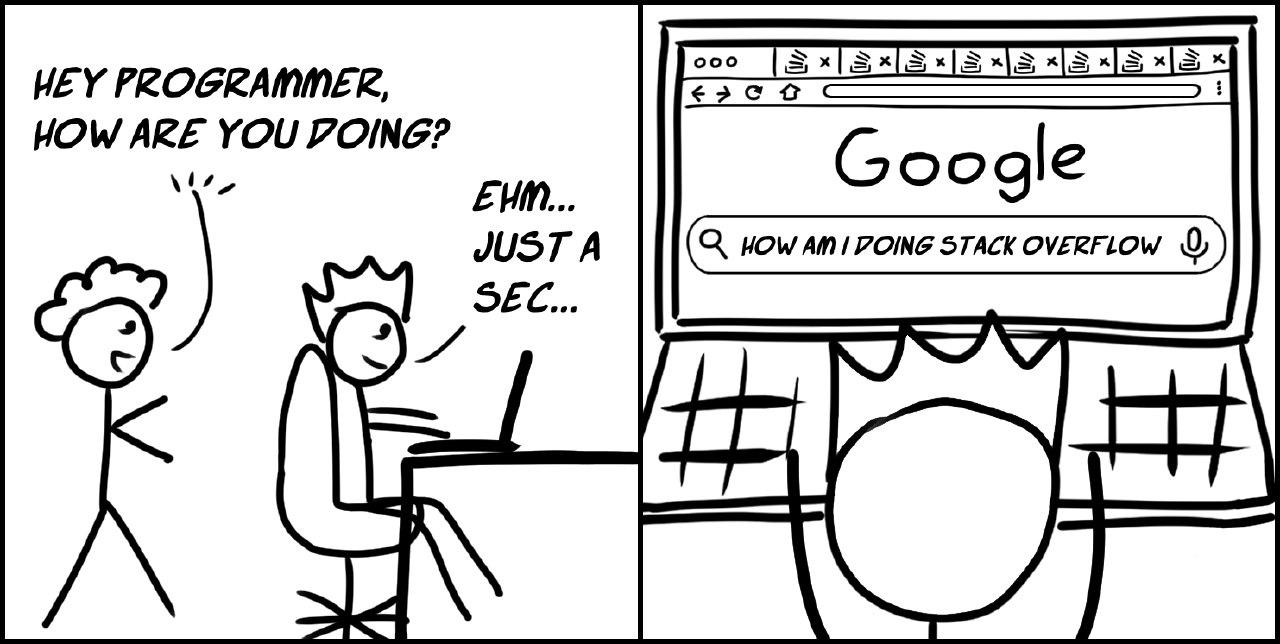
\includegraphics[width=0.6\linewidth ]{../Figures/stack-overflow.jpeg}
\end{figure}

\end{frame}




\begin{frame}
\frametitle{A bit about Python}
\begin{itemize}

\item Programming language intended for general-purpose high-level language
\item Web development, scientific and numeric education, desktop graphical user interface, software development
\item Free and open source 
\item You can do everything that you can do in a programming language
\item Big community (Google, Youtube, Nasa...)
\item High readability (more than R or C)
\item Python was first released in early 1980
\begin{itemize}

\item Python 2 in 2000 and Python 3 in 2008
\end{itemize}
\end{itemize}

\end{frame}
%----------------------------------------------------------------------------%
%----------------------------------------------------------------------------%

\begin{frame}
\frametitle{Black Holes and Python}
\begin{figure}

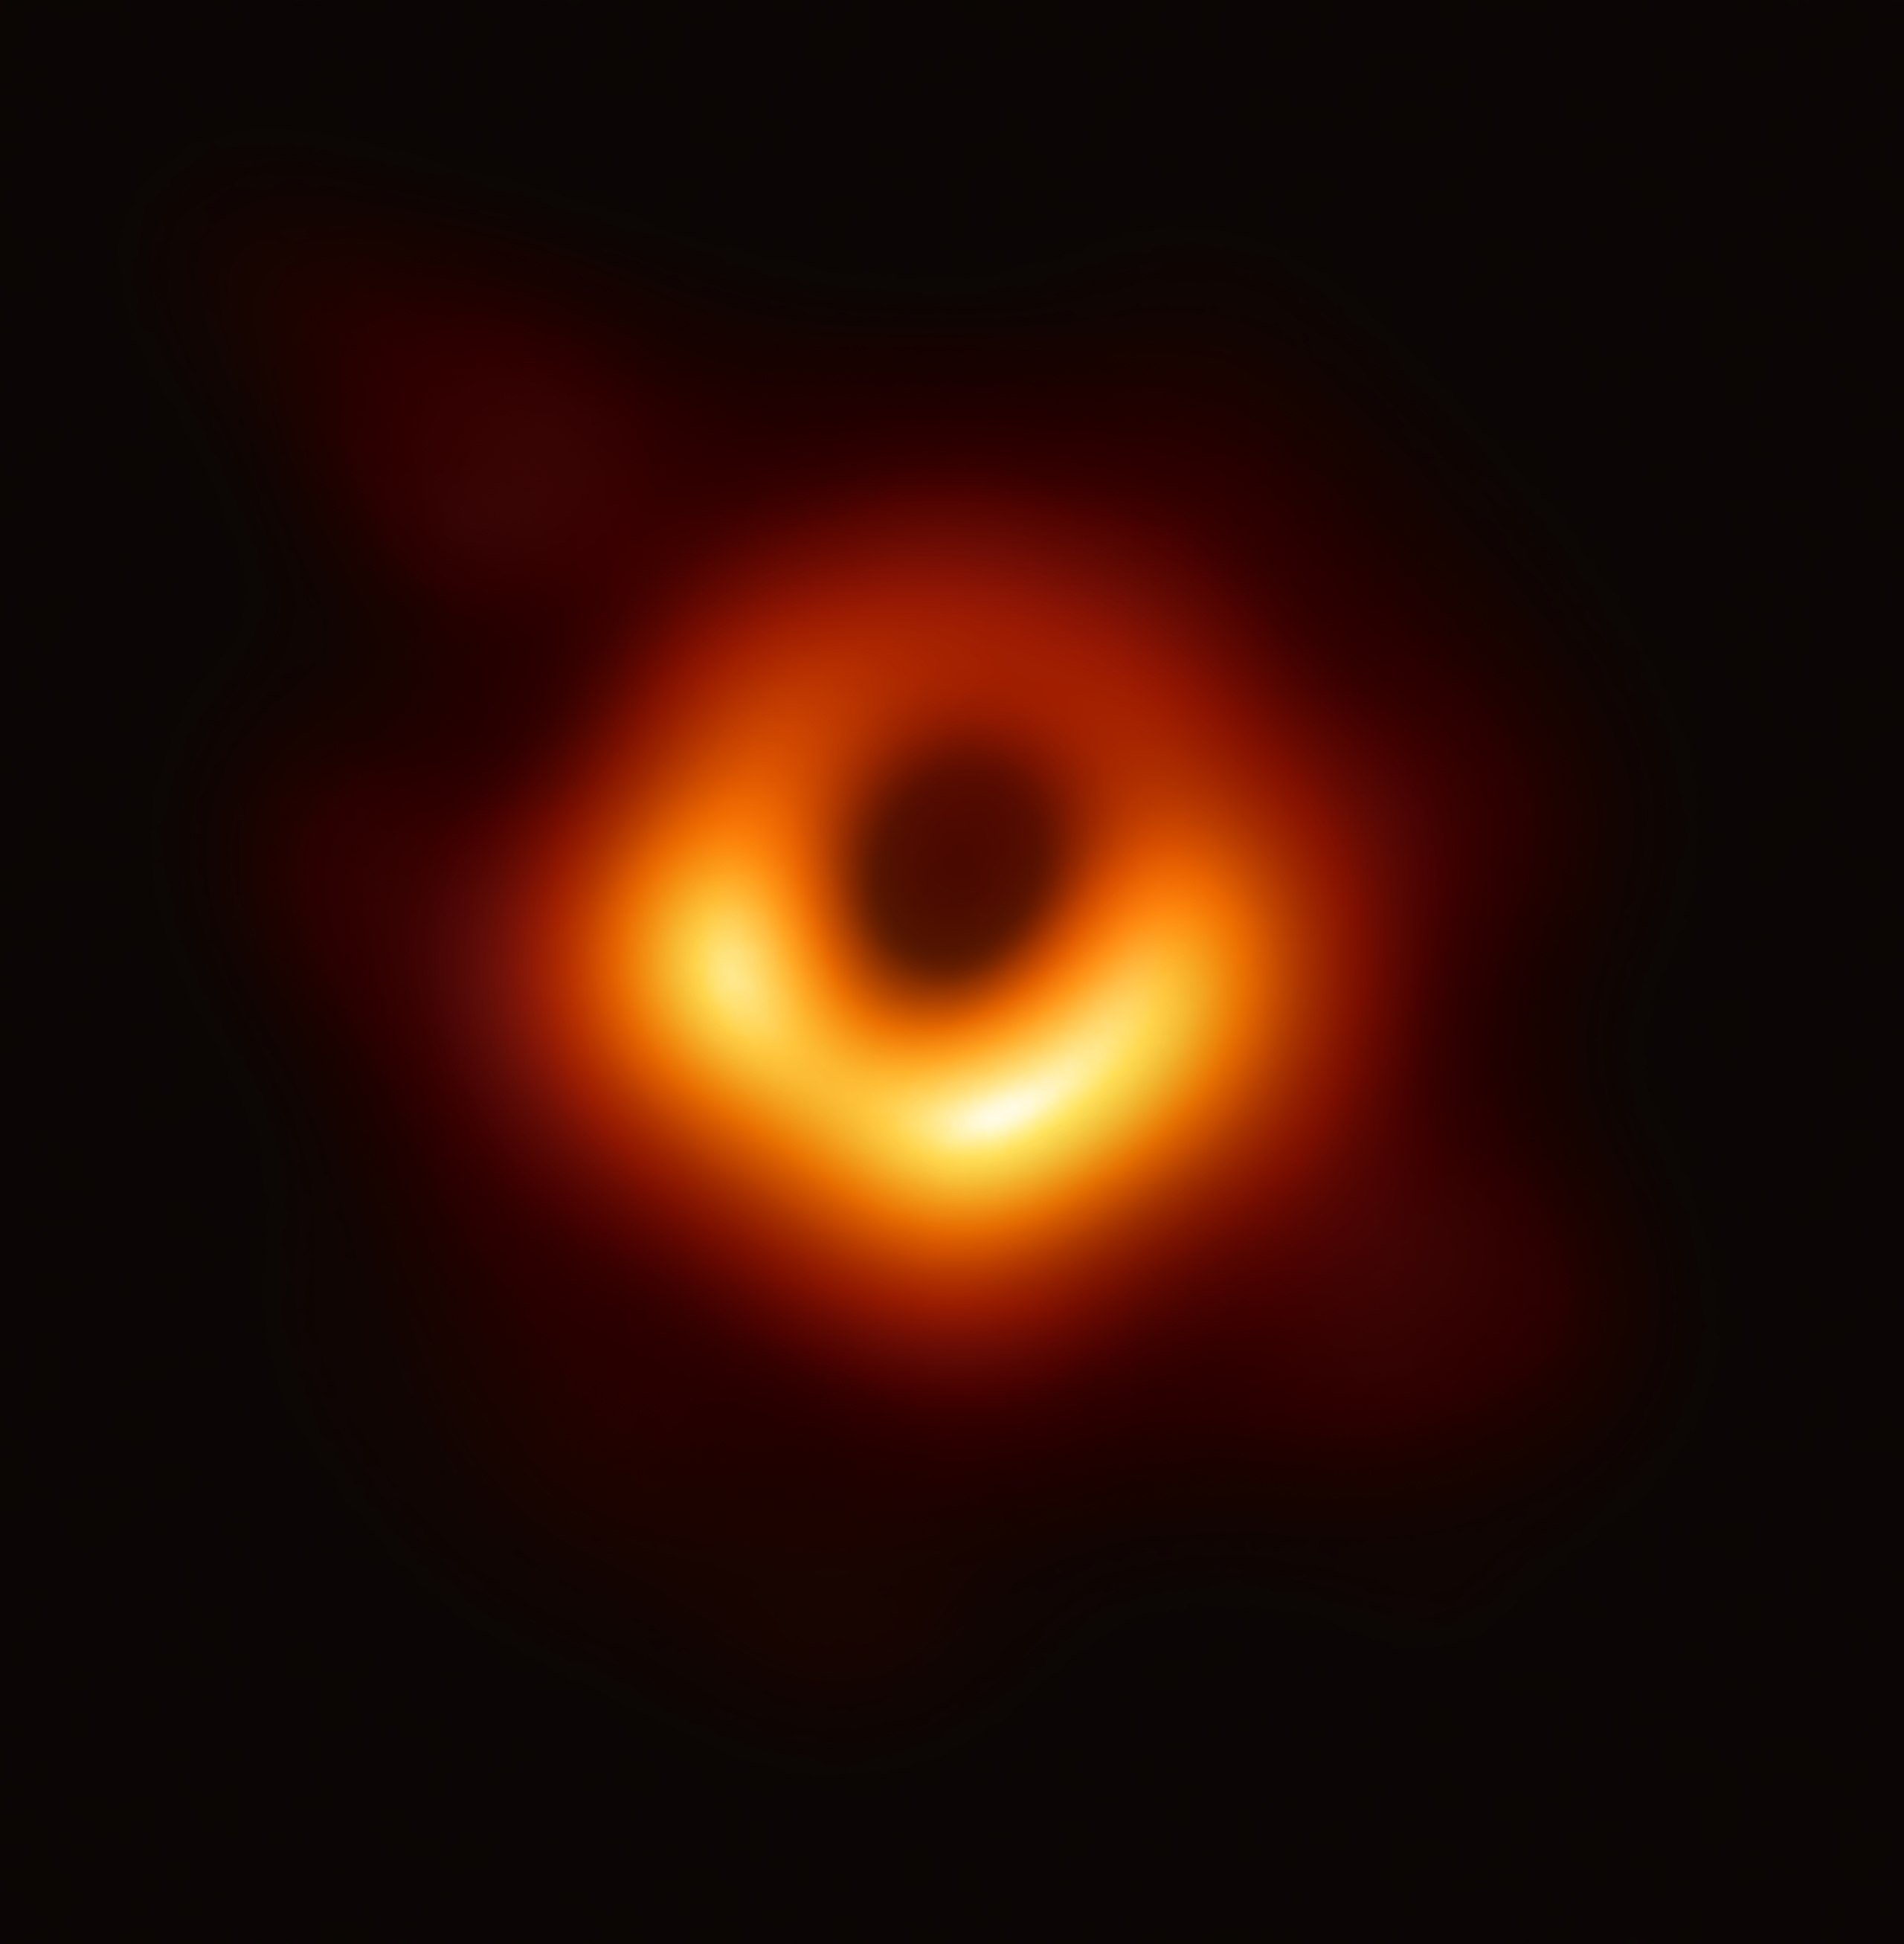
\includegraphics[width=0.5\linewidth ]{../Figures/black_hole.png}
\end{figure}

\end{frame}

%----------------------------------------------------------------------------%
\begin{frame}
\frametitle{Annoying things}
\begin{itemize}

\item Python 3 is not backward compatible with Python 2
\begin{itemize}
\item In this workshop we will use Python 3. Python 2 is not supported anymore
\item If you are starting a new project, do so in Python 3
\end{itemize}

\item Pandas Library (more on this next time)
\begin{itemize}
\item But very useful 
\end{itemize}
\item + some minor things we'll cover throughout the course 
\begin{itemize}

\item example: split() vs join()
\begin{itemize}
\item sentence = "We will rock you!"

\item words = sentence.split(" ") but sentence = " ".join(words) (?)
\end{itemize}


\end{itemize}

\end{itemize}

\end{frame}
%----------------------------------------------------------------------------%
\begin{frame}
\frametitle{Purpose of the worshop}
\begin{itemize}

\item Programming in Python, Natural Language Processing and Machine Learning tools are (mildly put) very broad topics, and we will not be able to cover many(!) things
\item Foundations concepts such that in the future you get confidence in starting to dig deeper into these topics
 
\end{itemize}

\end{frame}
%----------------------------------------------------------------------------%
\begin{frame}
\frametitle{Recommended Material}
\begin{itemize}
\item Python
\begin{itemize}

\item \href{https://www.codecademy.com/catalog/language/python}{\color{ blue}{Codecademy}} is the place to start
\item \href{https://automatetheboringstuff.com/}{\color{ blue}{Automate the Boring Stuff with Python}} and \href{https://realpython.com/}{\color{ blue}{The Real Python}} are great sources
%
\end{itemize}

\item Machine Learning 
\begin{itemize}

\item An Introduction to Statistical Learning (ISL) by Gareth, Witten,  Hastie and Tibshirani
\item  The Elements of Statistical Learning (ESL) by Hastie, Tibshirani, Friedman
\item  Statistical Learning with Sparsity (SLS) by Hastie, Tibshirani, Wainwright
\item  Introduction to Machine Learning with Python: A Guide for Data Scientists (IMLP) by Sarah Guido, and Andreas Muller
\end{itemize}

\item Natural Language Processing
\begin{itemize}

\item \href{https://nlp.stanford.edu/IR-book/information-retrieval-book.html}{\color{ blue}{Introduction to Information Retrieval}} by Christopher D. Manning, Prabhakar Raghavan and Hinrich Schutze

\item  Speech and Language Processing by Dan Jurafsky and James H. Martin
\end{itemize}
\end{itemize}

\end{frame}

%----------------------------------------------------------------------------%
\end{document}

